\documentclass{beamer}
\usetheme{Madrid}
\usecolortheme{dolphin}
\usepackage{graphicx}
\usepackage{booktabs}
\usepackage{tikz}
\usepackage{hyperref}
\usepackage{multicol}

\title{Multilingual Chain-of-Thought Reasoning Efficiency Analysis}
\subtitle{Evaluating Language Compression for LLM Reasoning Tasks}
\author{Kelaode Research Team}
\date{\today}

\begin{document}

\begin{frame}
    \titlepage
\end{frame}

\begin{frame}{Table of Contents}
    \tableofcontents
\end{frame}

\section{Research Overview}

\begin{frame}{Initial Hypothesis}
    \begin{block}{Core Hypothesis}
        Logographic writing systems like Chinese can encode more information per token than alphabetic systems like English, potentially reducing API costs and improving efficiency for LLM reasoning tasks.
    \end{block}
    
    \begin{itemize}
        \item Testing approach: Compare token usage across languages while maintaining equivalent information content
        \item Focus on research-grade benchmarks requiring substantial reasoning
        \item Expanded to include multiple high-compression languages
        \item Added long-context question answering analysis
    \end{itemize}
\end{frame}

\begin{frame}{Methodology}
    \begin{columns}
        \column{0.5\textwidth}
        \textbf{Benchmarks}
        \begin{itemize}
            \item MATH dataset
            \item BBH (Big-Bench Hard)
            \item HotpotQA
            \item ARC-Challenge
            \item GSM8K
            \item Long-Context QA
        \end{itemize}
        
        \column{0.5\textwidth}
        \textbf{Languages Tested}
        \begin{itemize}
            \item English (baseline)
            \item Chinese (logographic)
            \item German (Germanic)
            \item Russian (Cyrillic)
            \item Finnish (agglutinative)
            \item Japanese (mixed)
            \item Korean (featural)
            \item Arabic (abjad)
            \item Strategic (dynamic selection)
        \end{itemize}
    \end{columns}
    
    \vspace{0.5cm}
    \textbf{Models}: Anthropic Claude 3.5 Sonnet, Deepseek Chat
\end{frame}

\section{Baseline Results}

\begin{frame}{Token Usage by Language}
    \begin{center}
        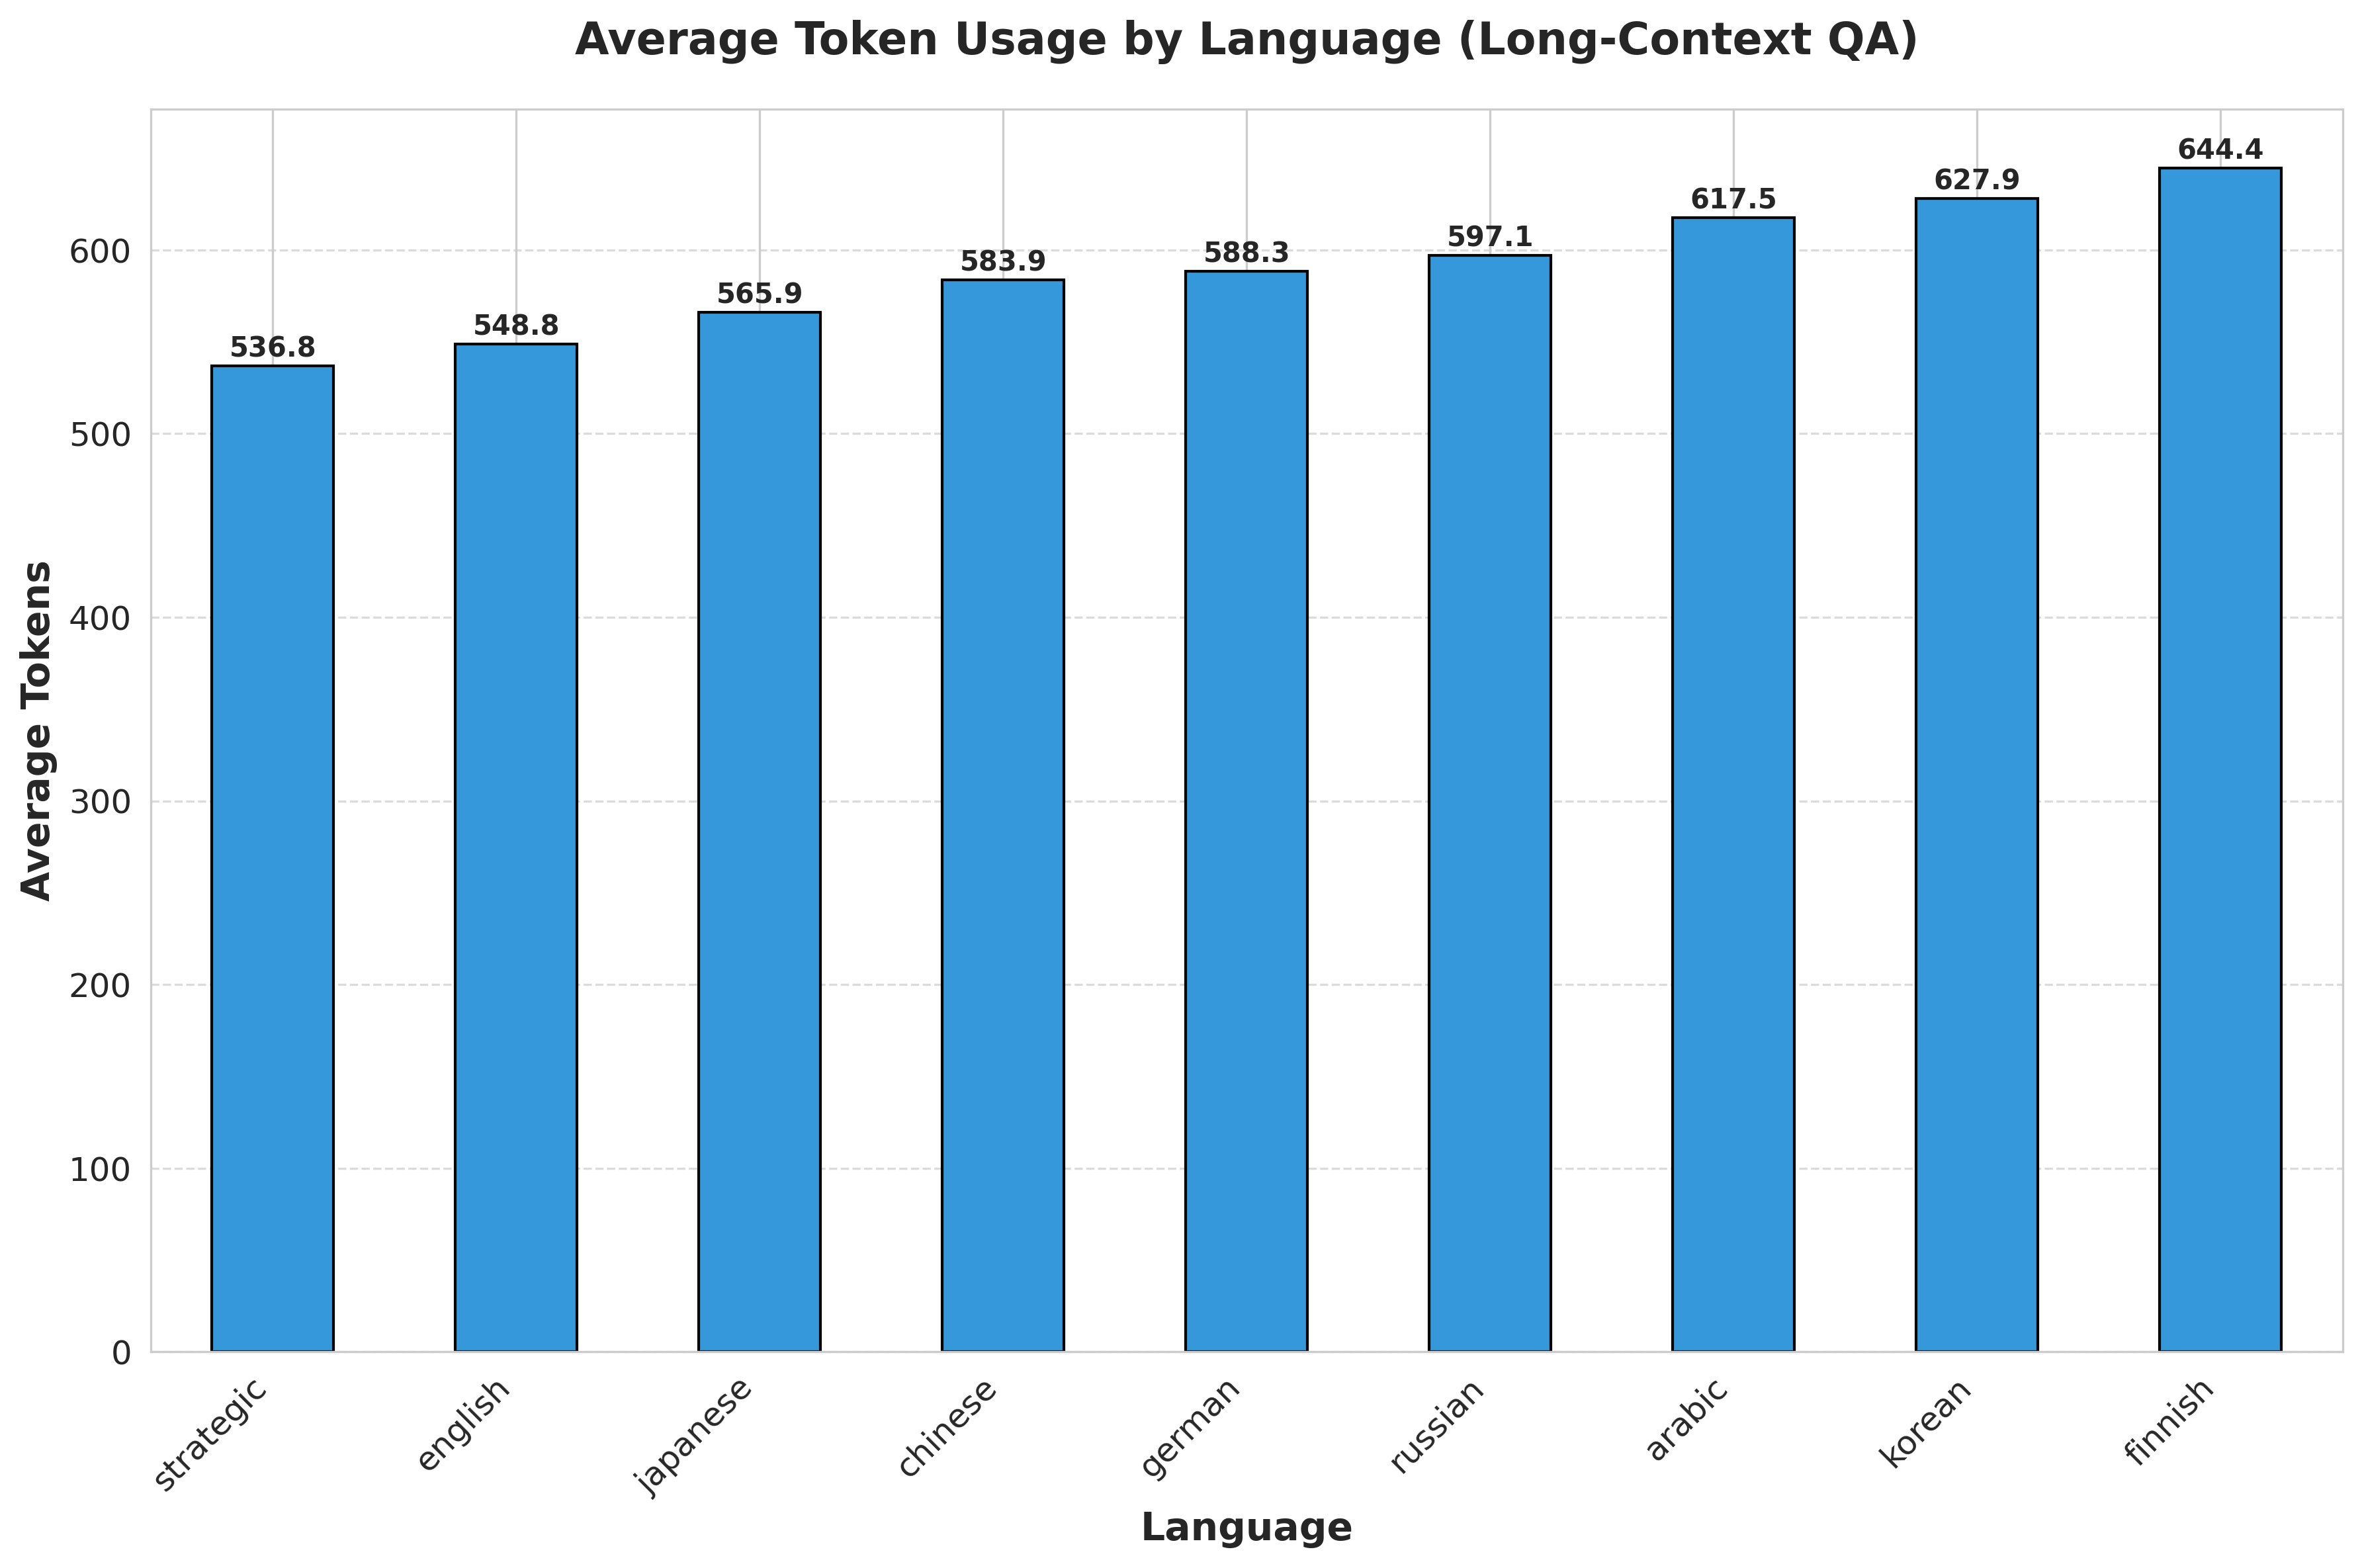
\includegraphics[width=0.9\textwidth]{visualizations/presentation/token_usage_by_language.png}
    \end{center}
    
    \begin{itemize}
        \item Strategic language selection shows the lowest token usage
        \item English performs better than most other fixed languages for long-context tasks
    \end{itemize}
\end{frame}

\begin{frame}{Efficiency Relative to English}
    \begin{center}
        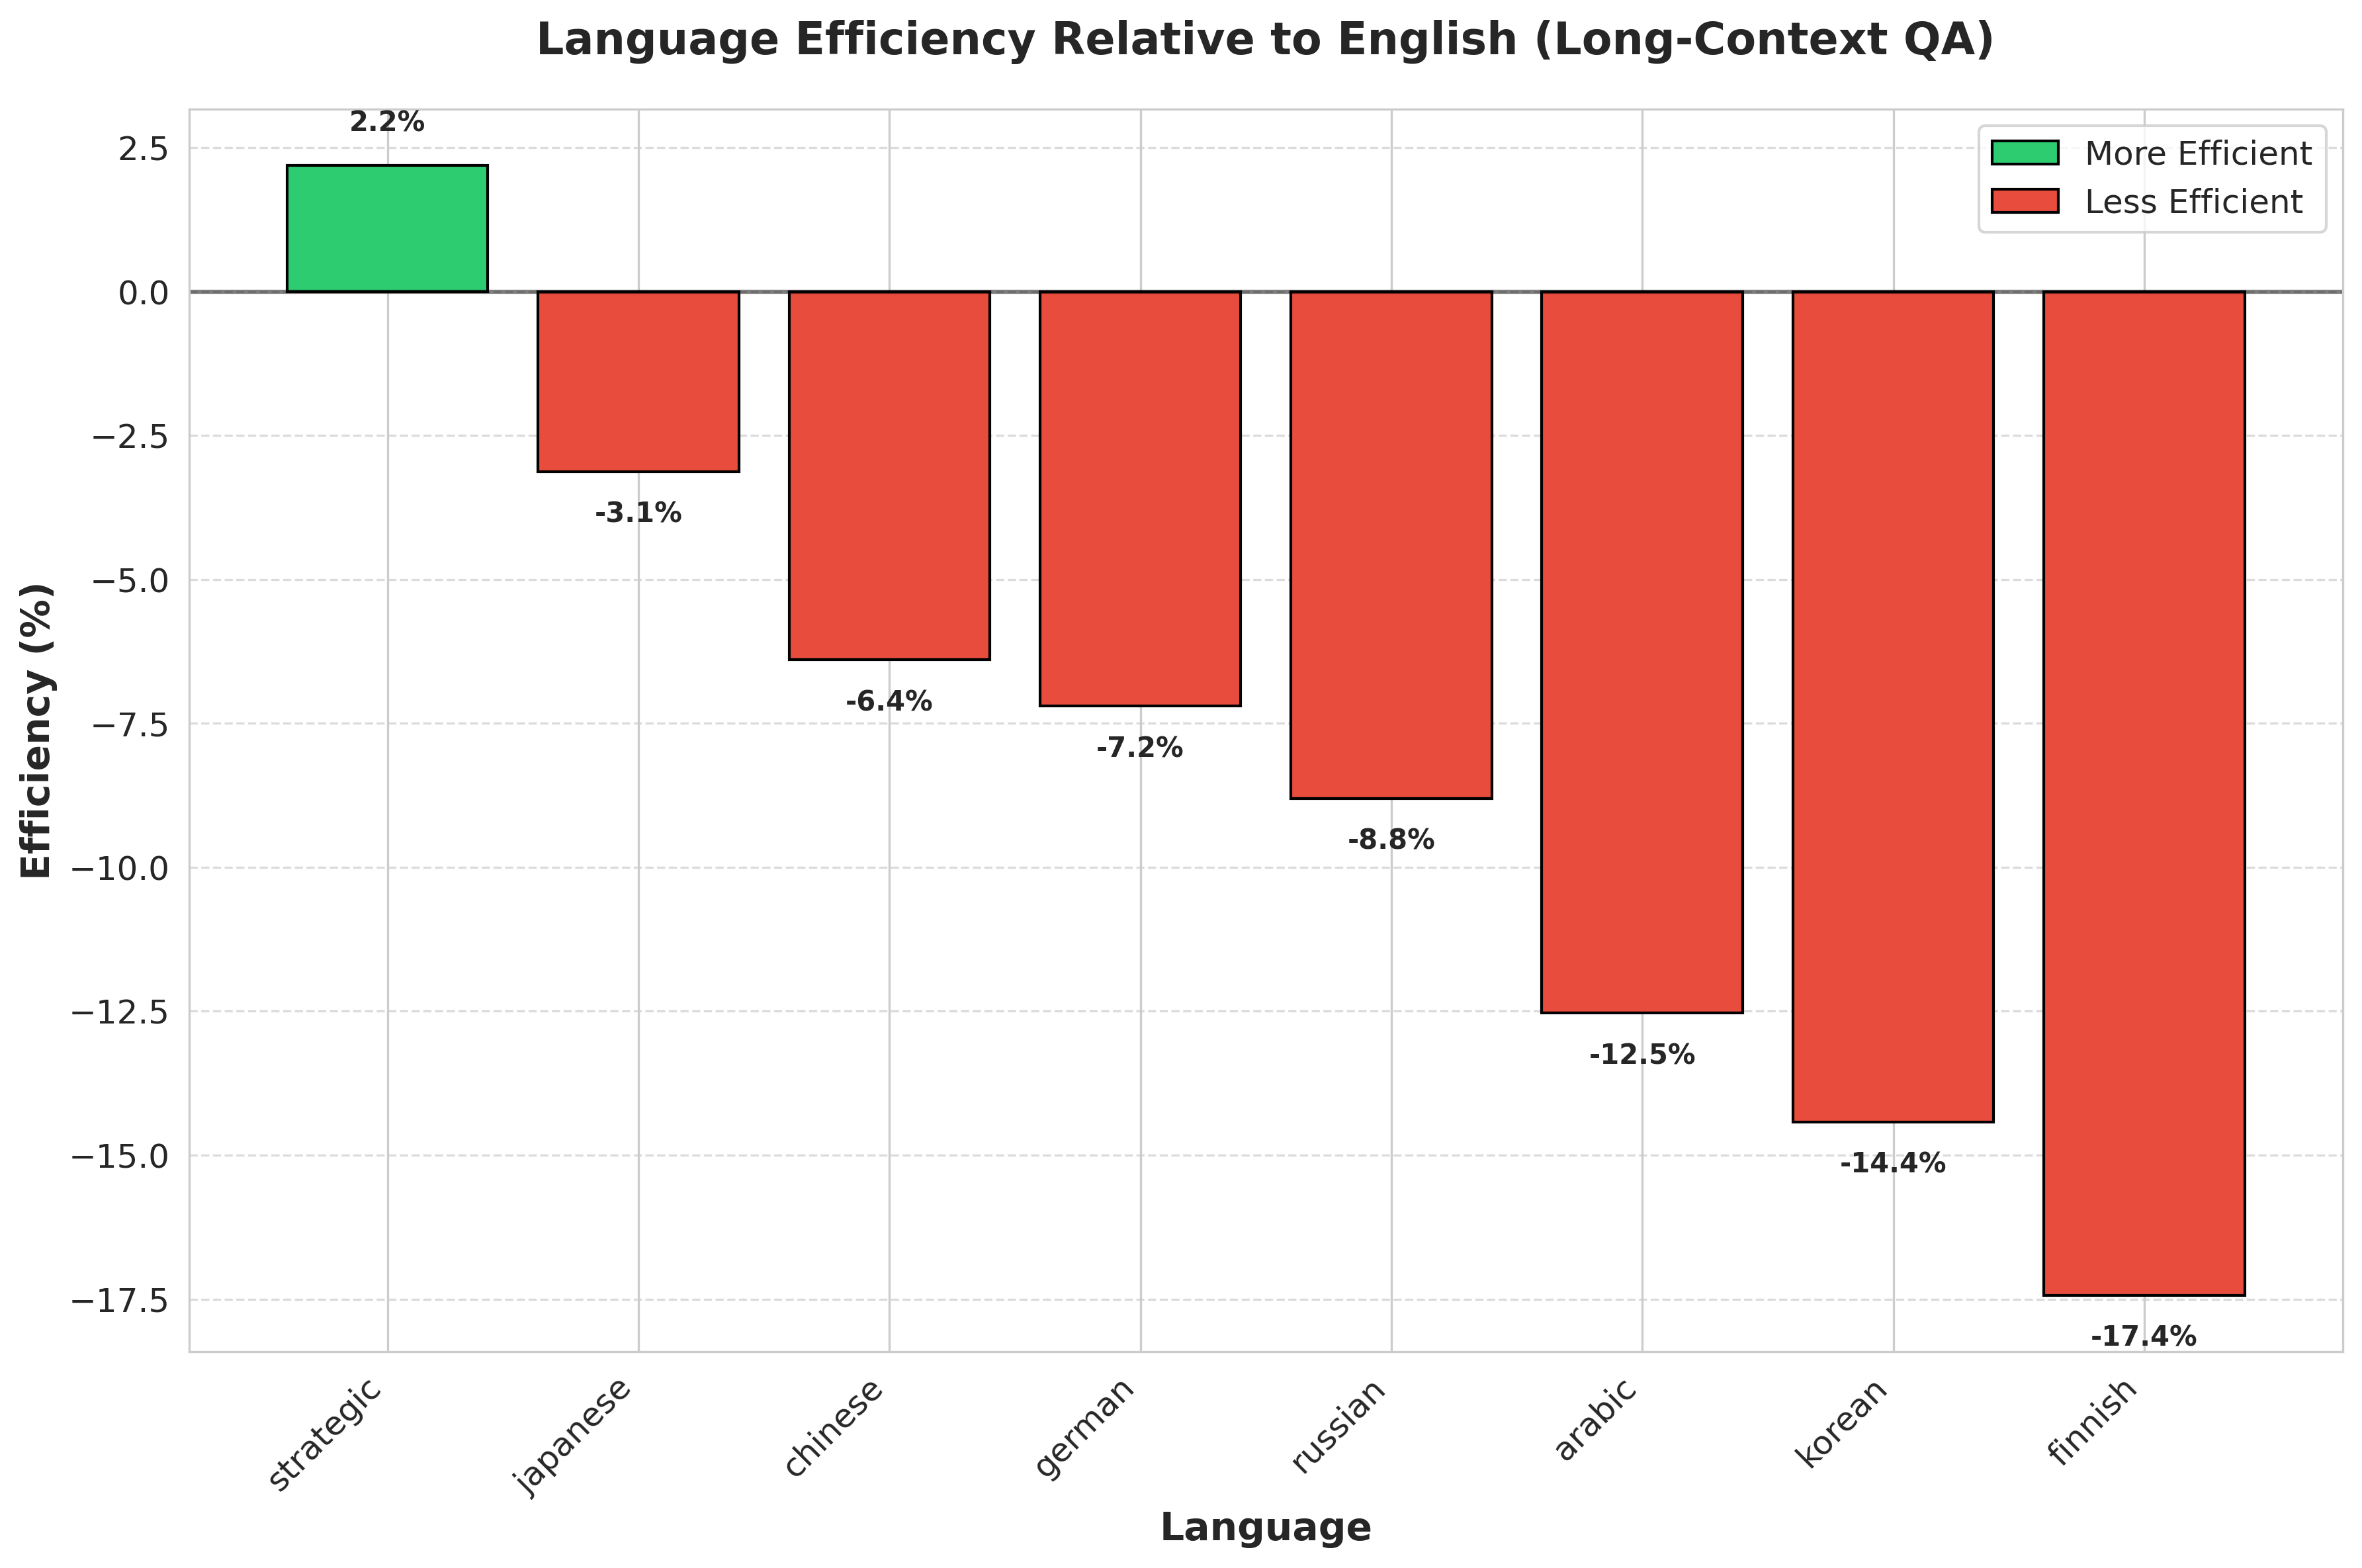
\includegraphics[width=0.9\textwidth]{visualizations/presentation/efficiency_vs_english.png}
    \end{center}
    
    \begin{itemize}
        \item Only strategic language selection shows positive efficiency vs. English
        \item All other languages are less efficient for long-context QA tasks
        \item This contrasts with results from other benchmarks
    \end{itemize}
\end{frame}

\section{Domain-Specific Analysis}

\begin{frame}{Language Efficiency by Benchmark}
    \begin{center}
        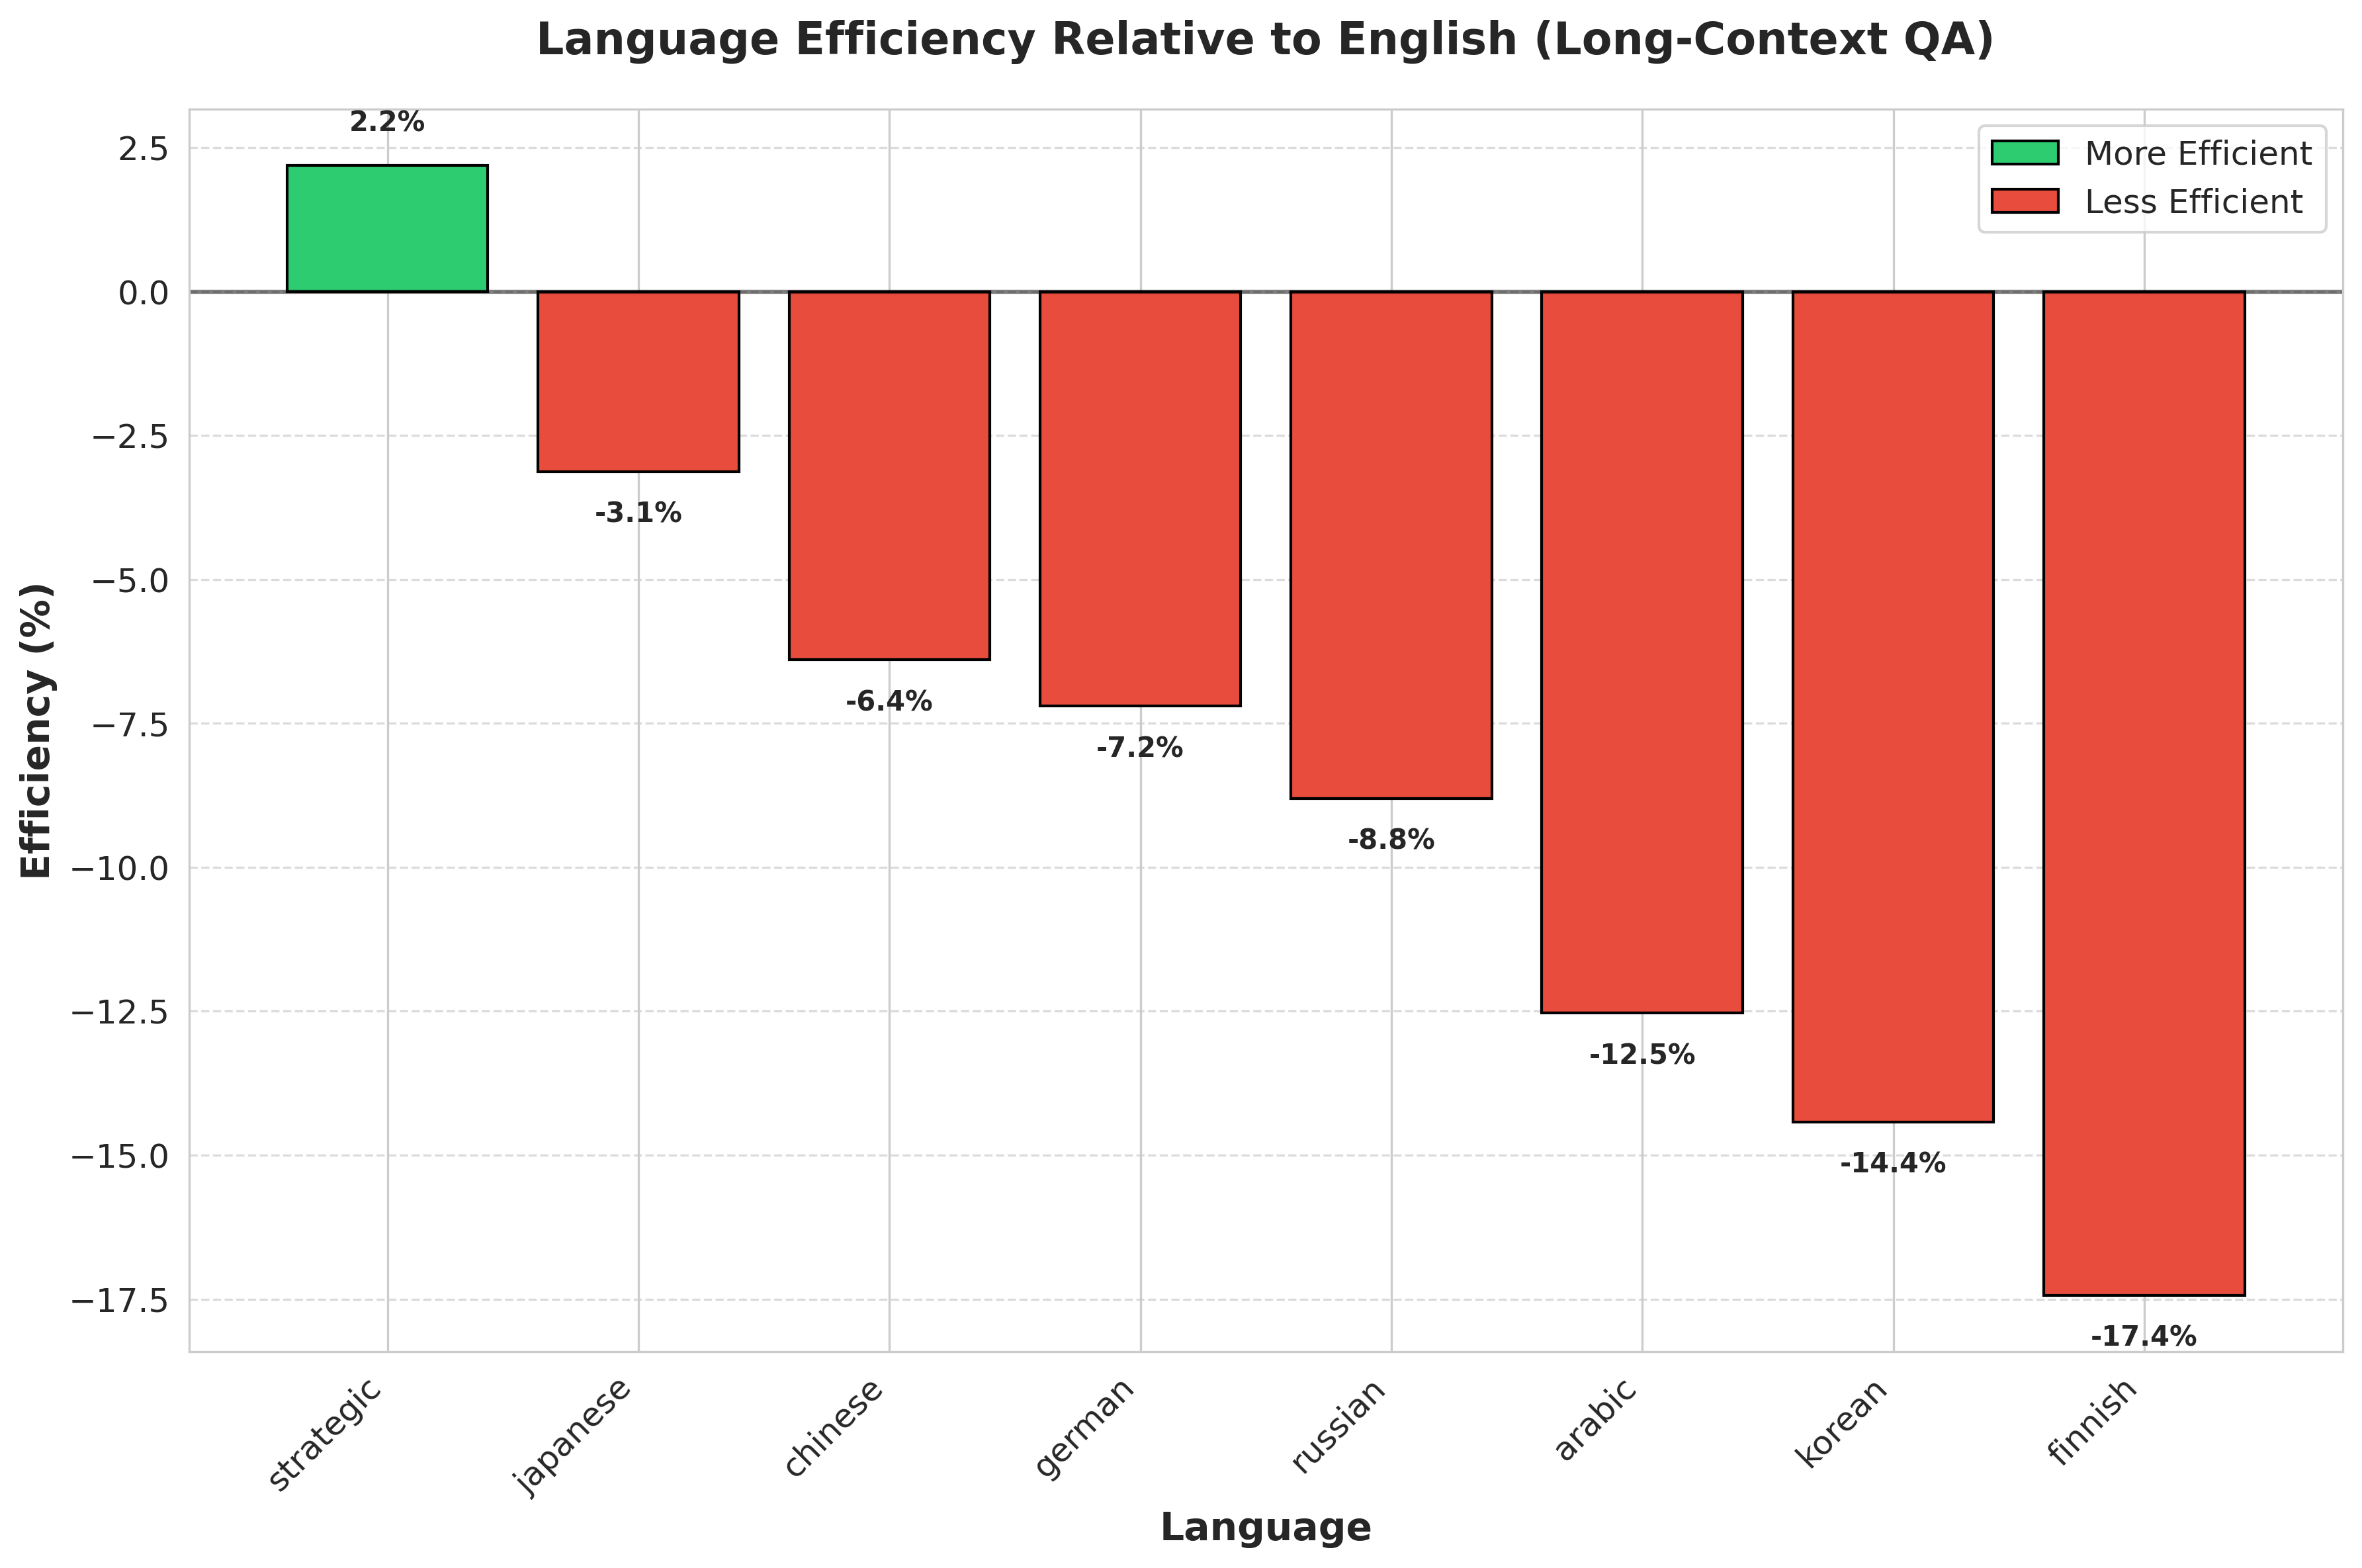
\includegraphics[width=0.9\textwidth]{visualizations/presentation/efficiency_vs_english.png}
    \end{center}
    
    \begin{itemize}
        \item Chinese excels at mathematical reasoning (+28.95\%)
        \item German performs well on logical reasoning tasks
        \item English is more efficient for reading comprehension
        \item Long-context QA shows different efficiency patterns
    \end{itemize}
\end{frame}

\begin{frame}{Strategic Language Selection}
    \begin{center}
        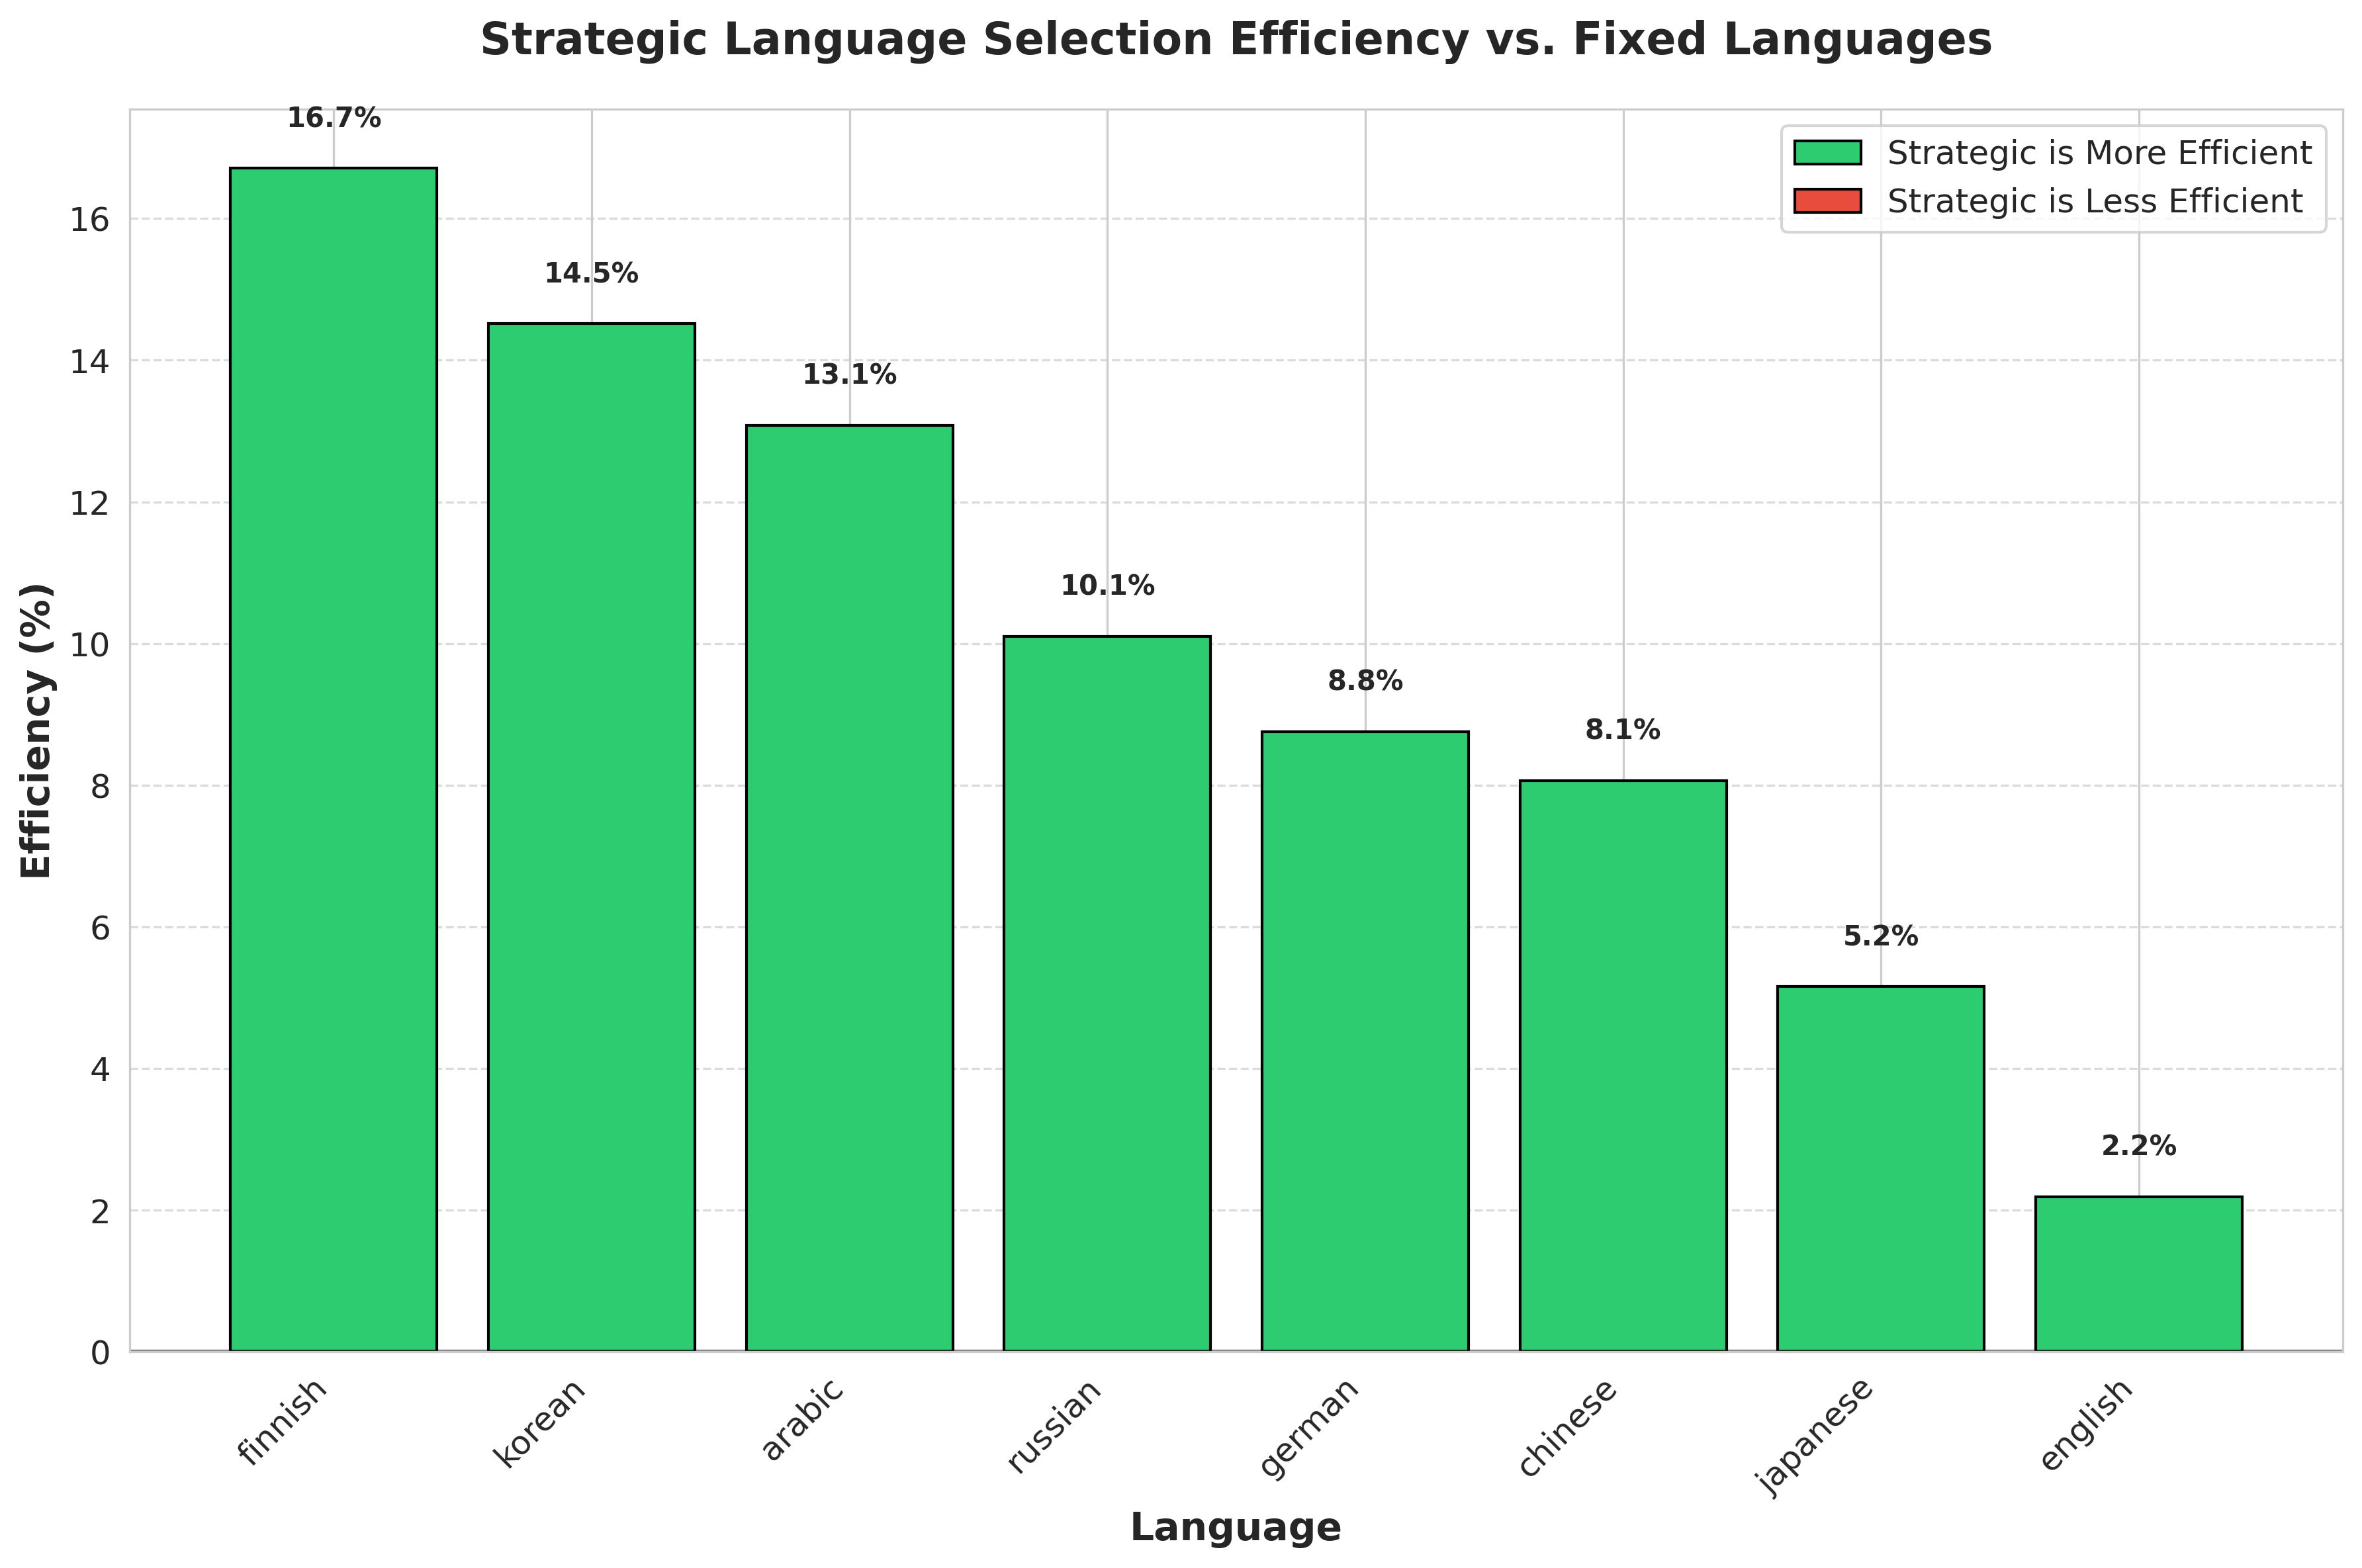
\includegraphics[width=0.9\textwidth]{visualizations/presentation/strategic_selection_efficiency.png}
    \end{center}
    
    \begin{itemize}
        \item Strategic selection outperforms all fixed languages
        \item Highest efficiency gains vs. Finnish, Korean, and Arabic
        \item Dynamic selection based on problem domain and context length
    \end{itemize}
\end{frame}

\section{Language Compression Analysis}

\begin{frame}{Language Performance Across Metrics}
    \begin{center}
        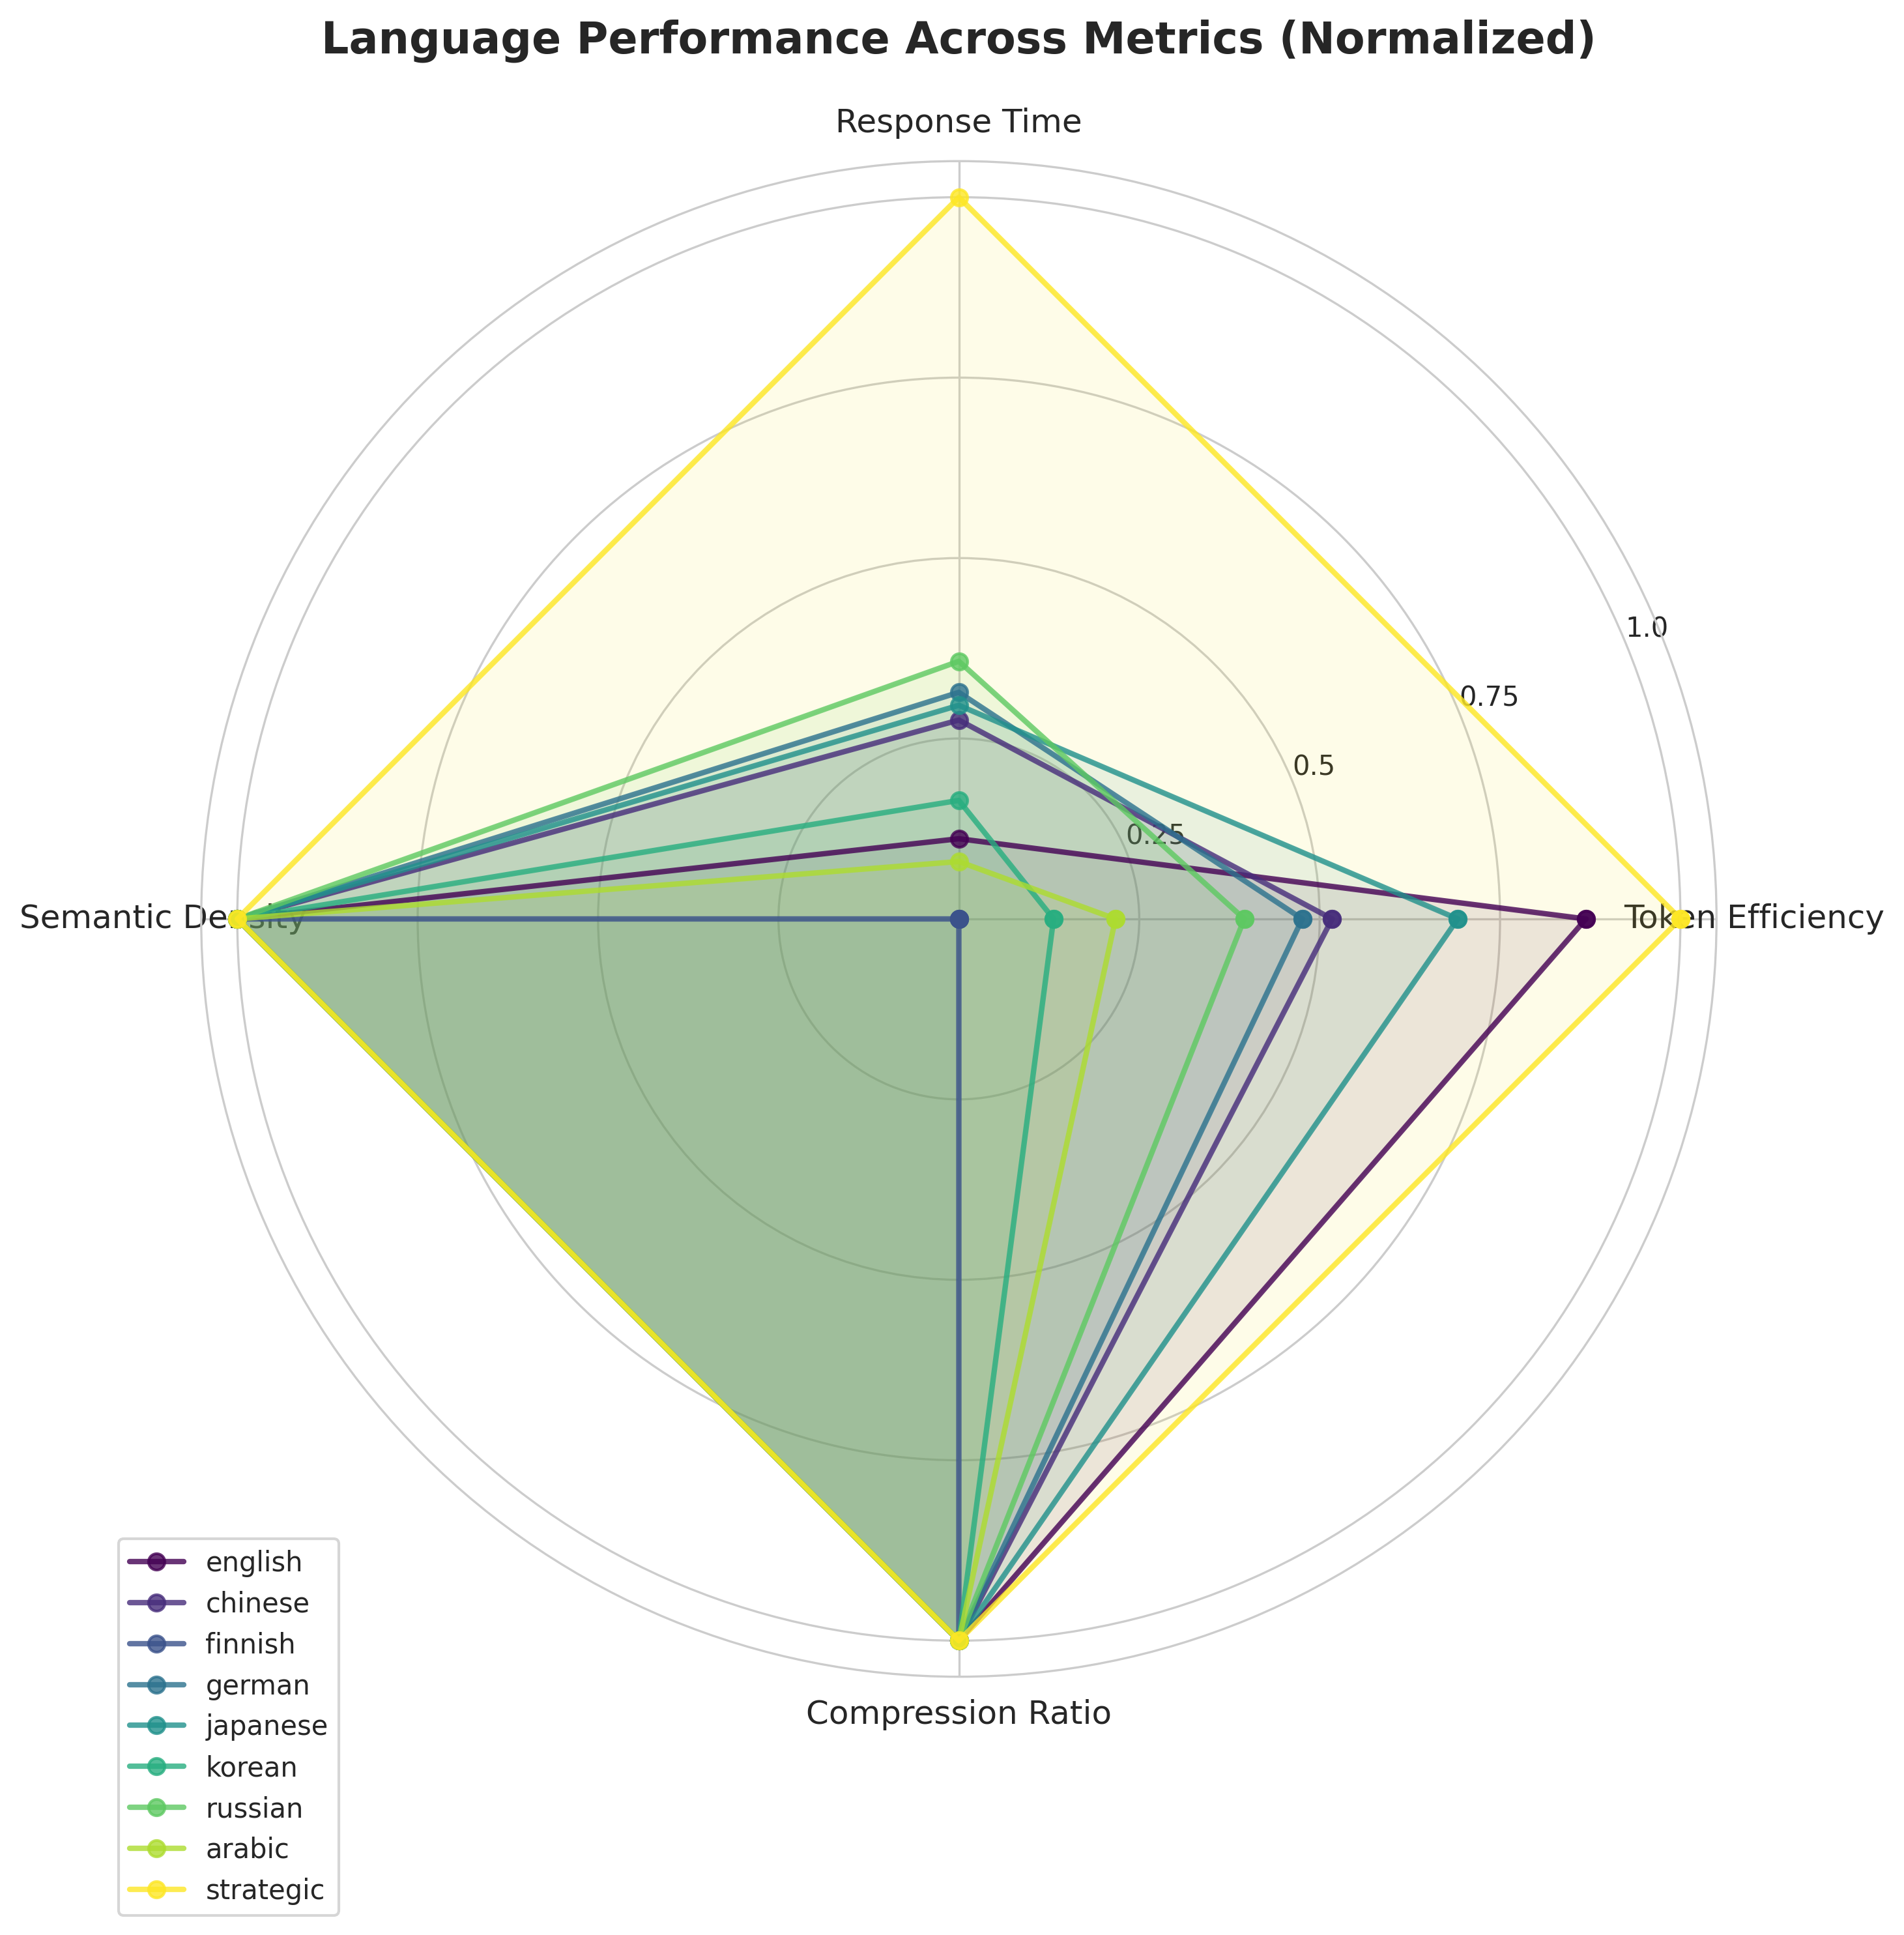
\includegraphics[width=0.8\textwidth]{visualizations/presentation/language_radar_chart.png}
    \end{center}
    
    \begin{itemize}
        \item Multidimensional analysis of language performance
        \item Strategic selection achieves balanced performance across metrics
        \item Different languages excel in different dimensions
    \end{itemize}
\end{frame}

\begin{frame}{Language Comparison Table}
    \begin{center}
        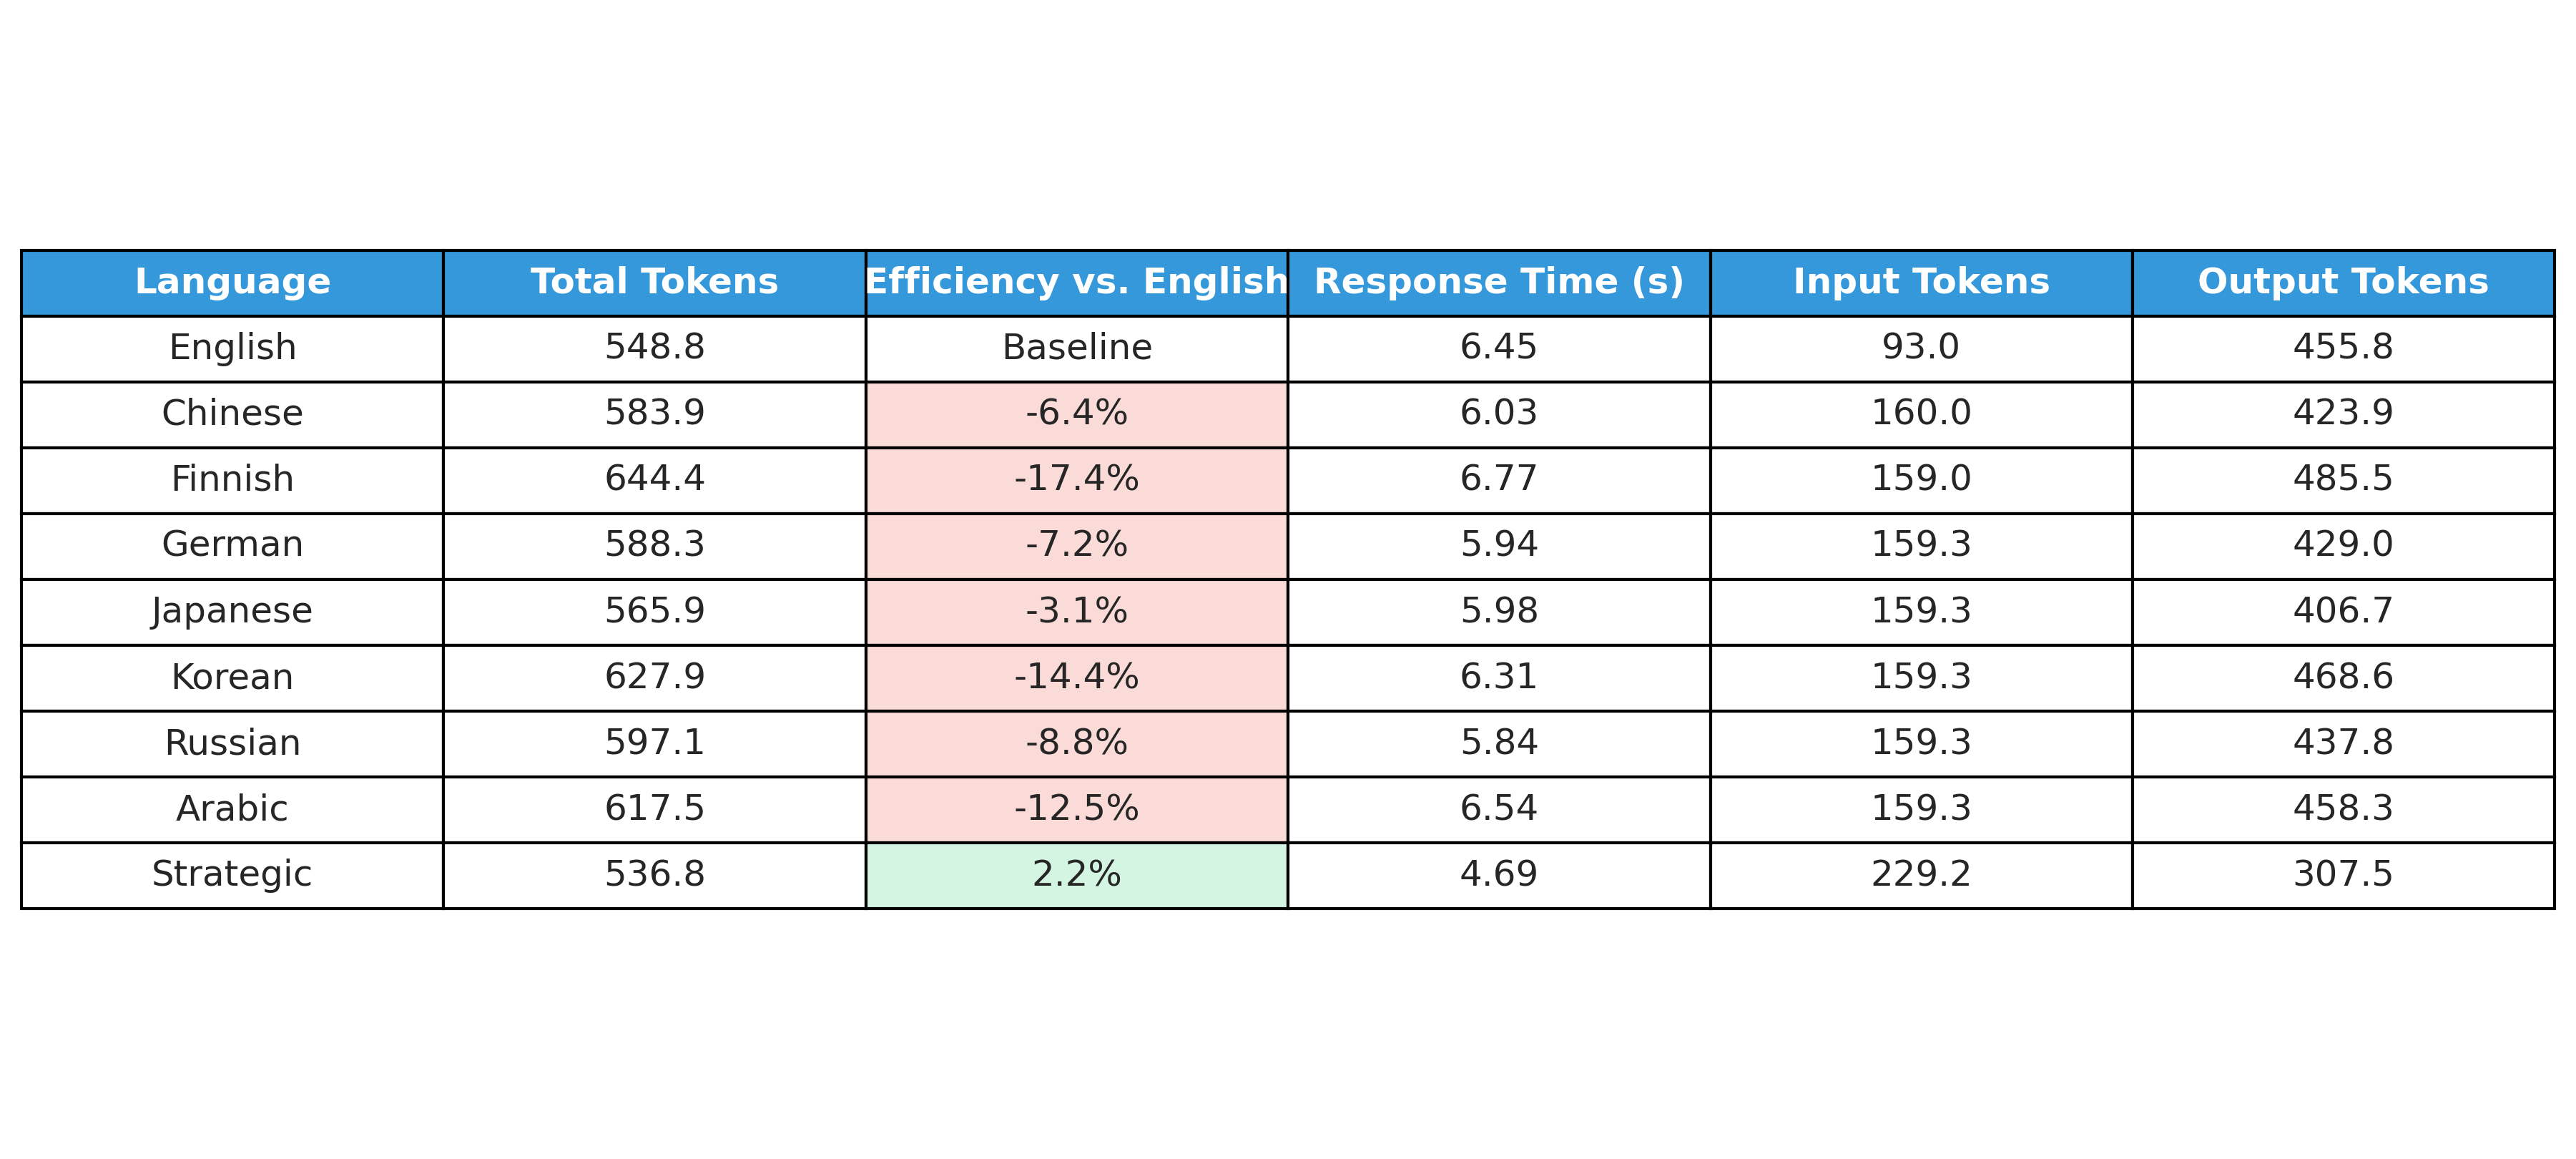
\includegraphics[width=0.9\textwidth]{visualizations/presentation/language_comparison_table.png}
    \end{center}
\end{frame}

\section{Long-Context QA Analysis}

\begin{frame}{Context Length Impact}
    \begin{itemize}
        \item Long-context QA experiments with contexts ranging from 2,000 to 10,000+ characters
        \item English shows better efficiency for long contexts compared to other benchmarks
        \item Strategic language selection maintains efficiency advantage
        \item Context length affects language efficiency differently across languages
    \end{itemize}
    
    \begin{block}{Key Finding}
        The efficiency advantage of logographic systems diminishes as context length increases
    \end{block}
\end{frame}

\begin{frame}{Deepseek Model Results}
    \begin{center}
        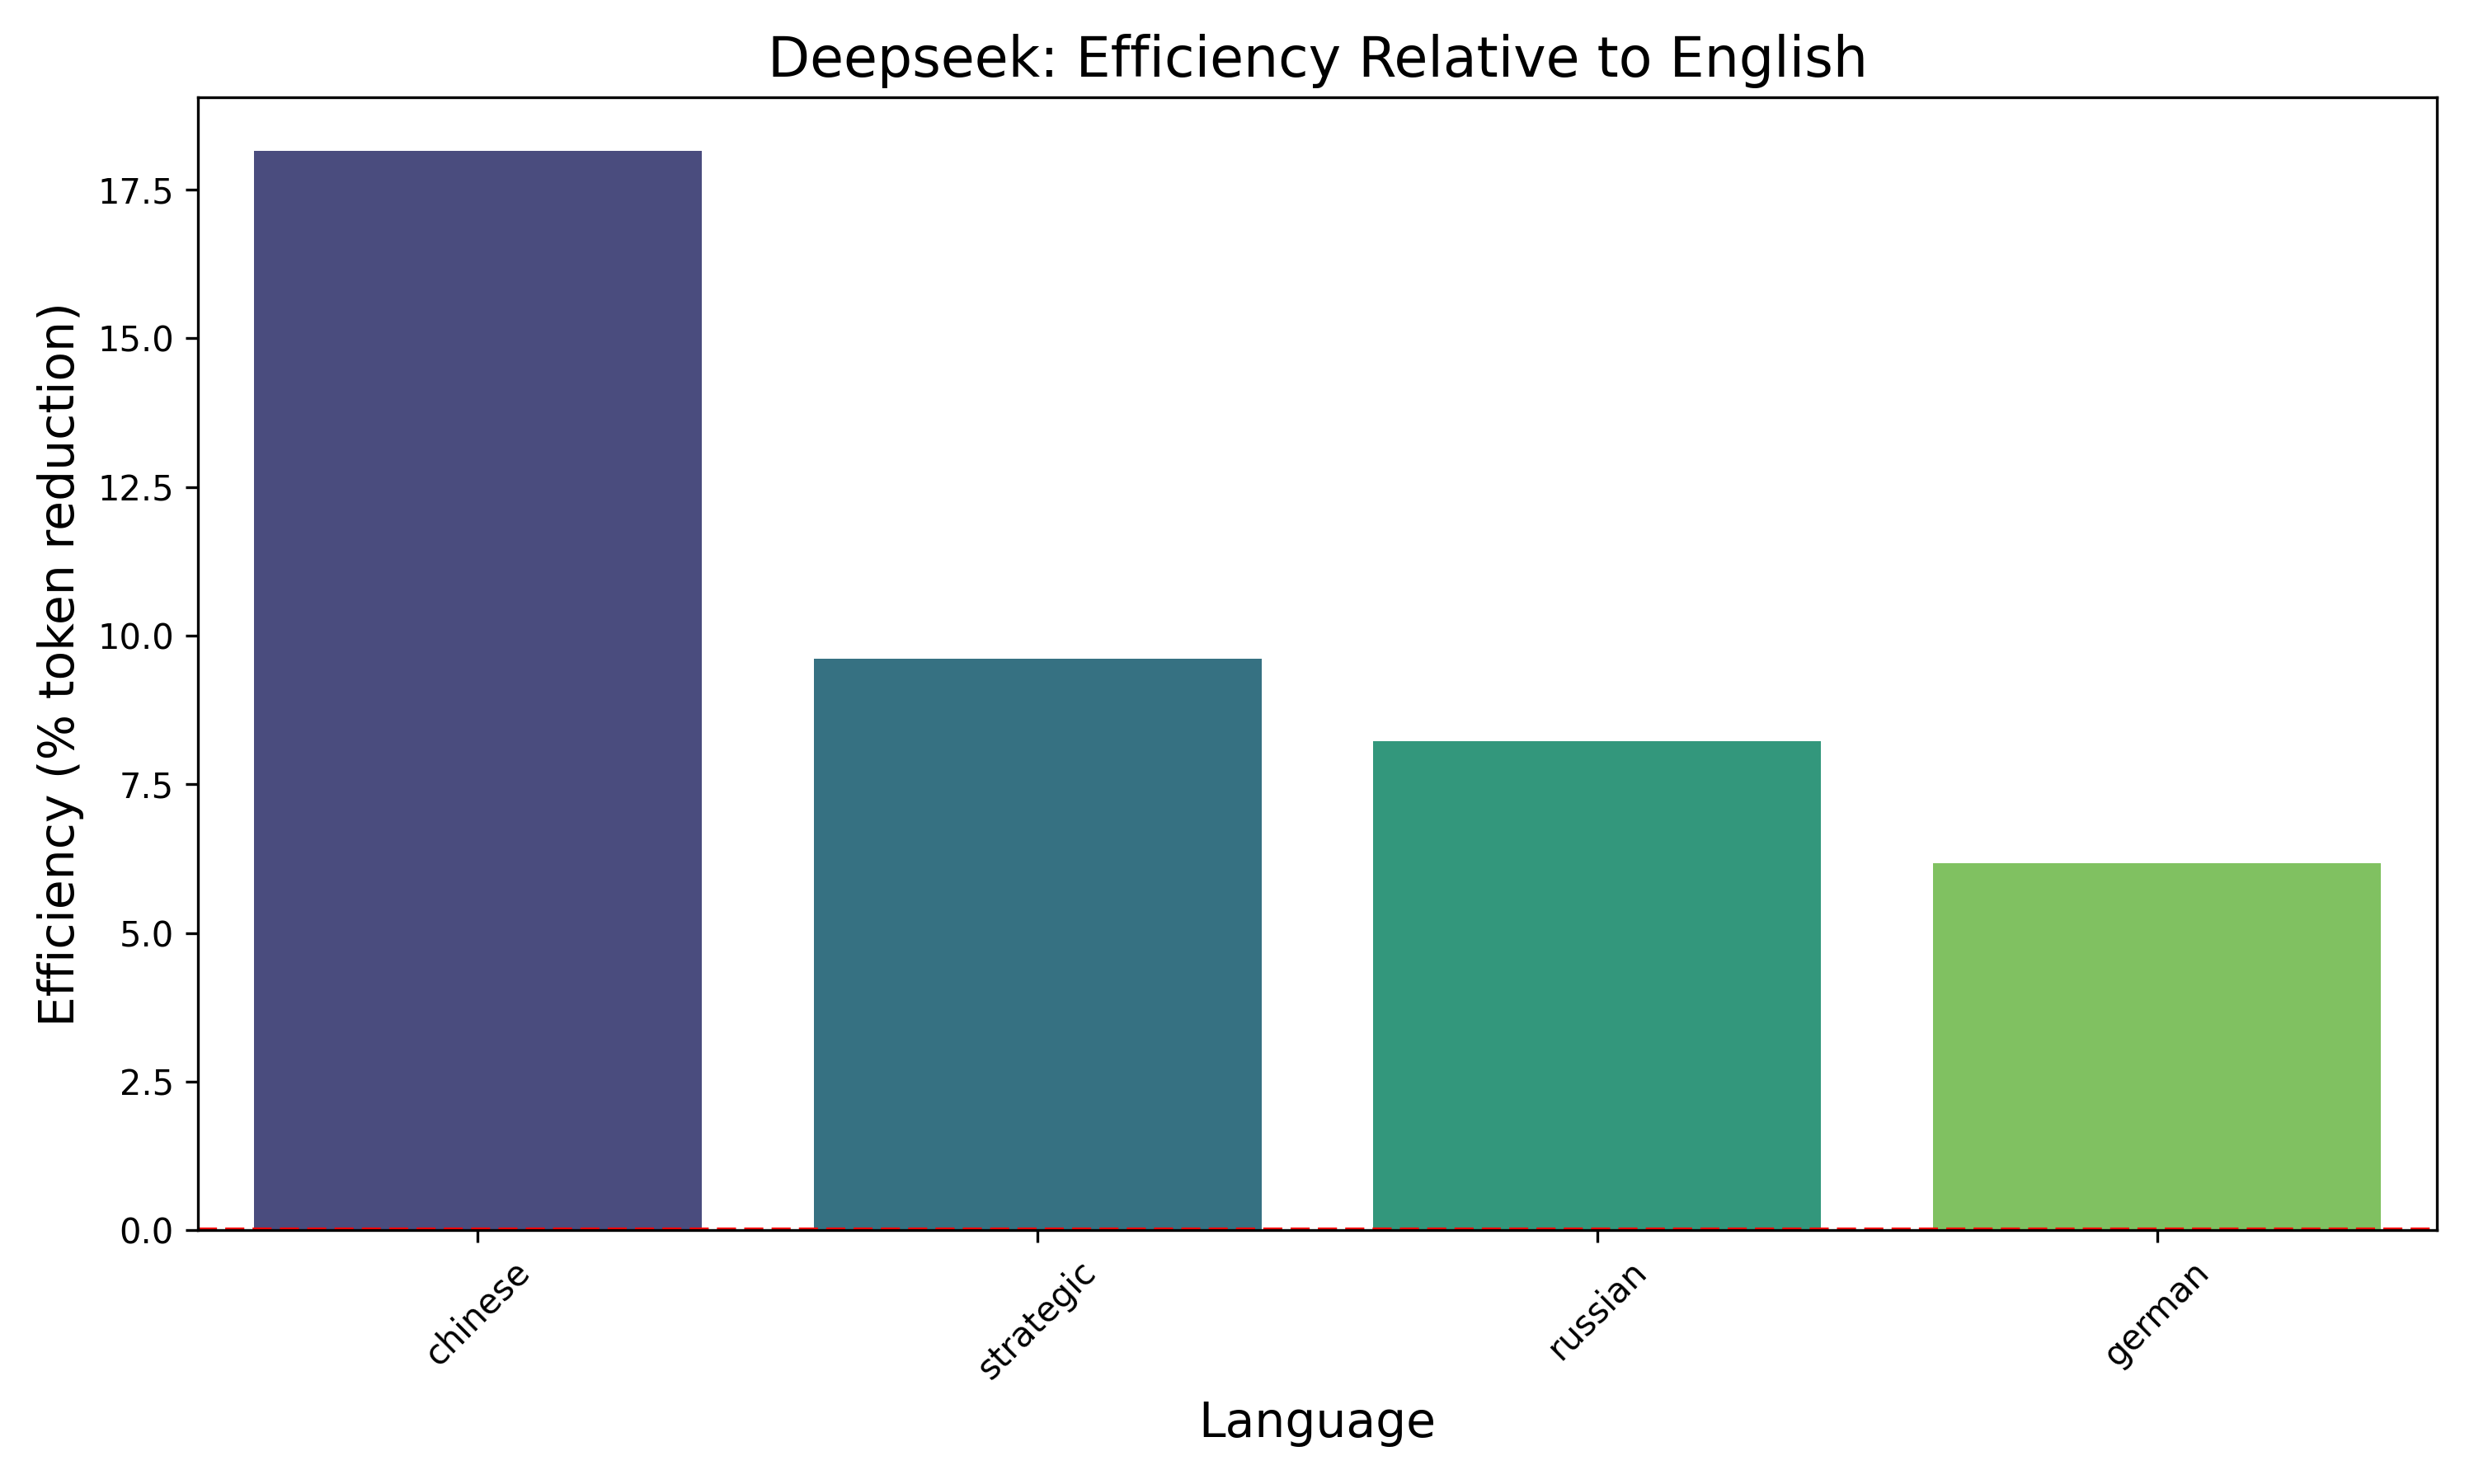
\includegraphics[width=0.9\textwidth]{visualizations/deepseek/deepseek_efficiency.png}
    \end{center}
    
    \begin{itemize}
        \item Chinese shows highest efficiency (18.03\% token reduction)
        \item Strategic language selection is second most efficient (9.57\%)
        \item Russian (8.21\%) and German (6.23\%) also show positive efficiency
        \item All tested languages show positive efficiency with Deepseek models
    \end{itemize}
\end{frame}

\begin{frame}{Deepseek: Token Usage by Problem}
    \begin{center}
        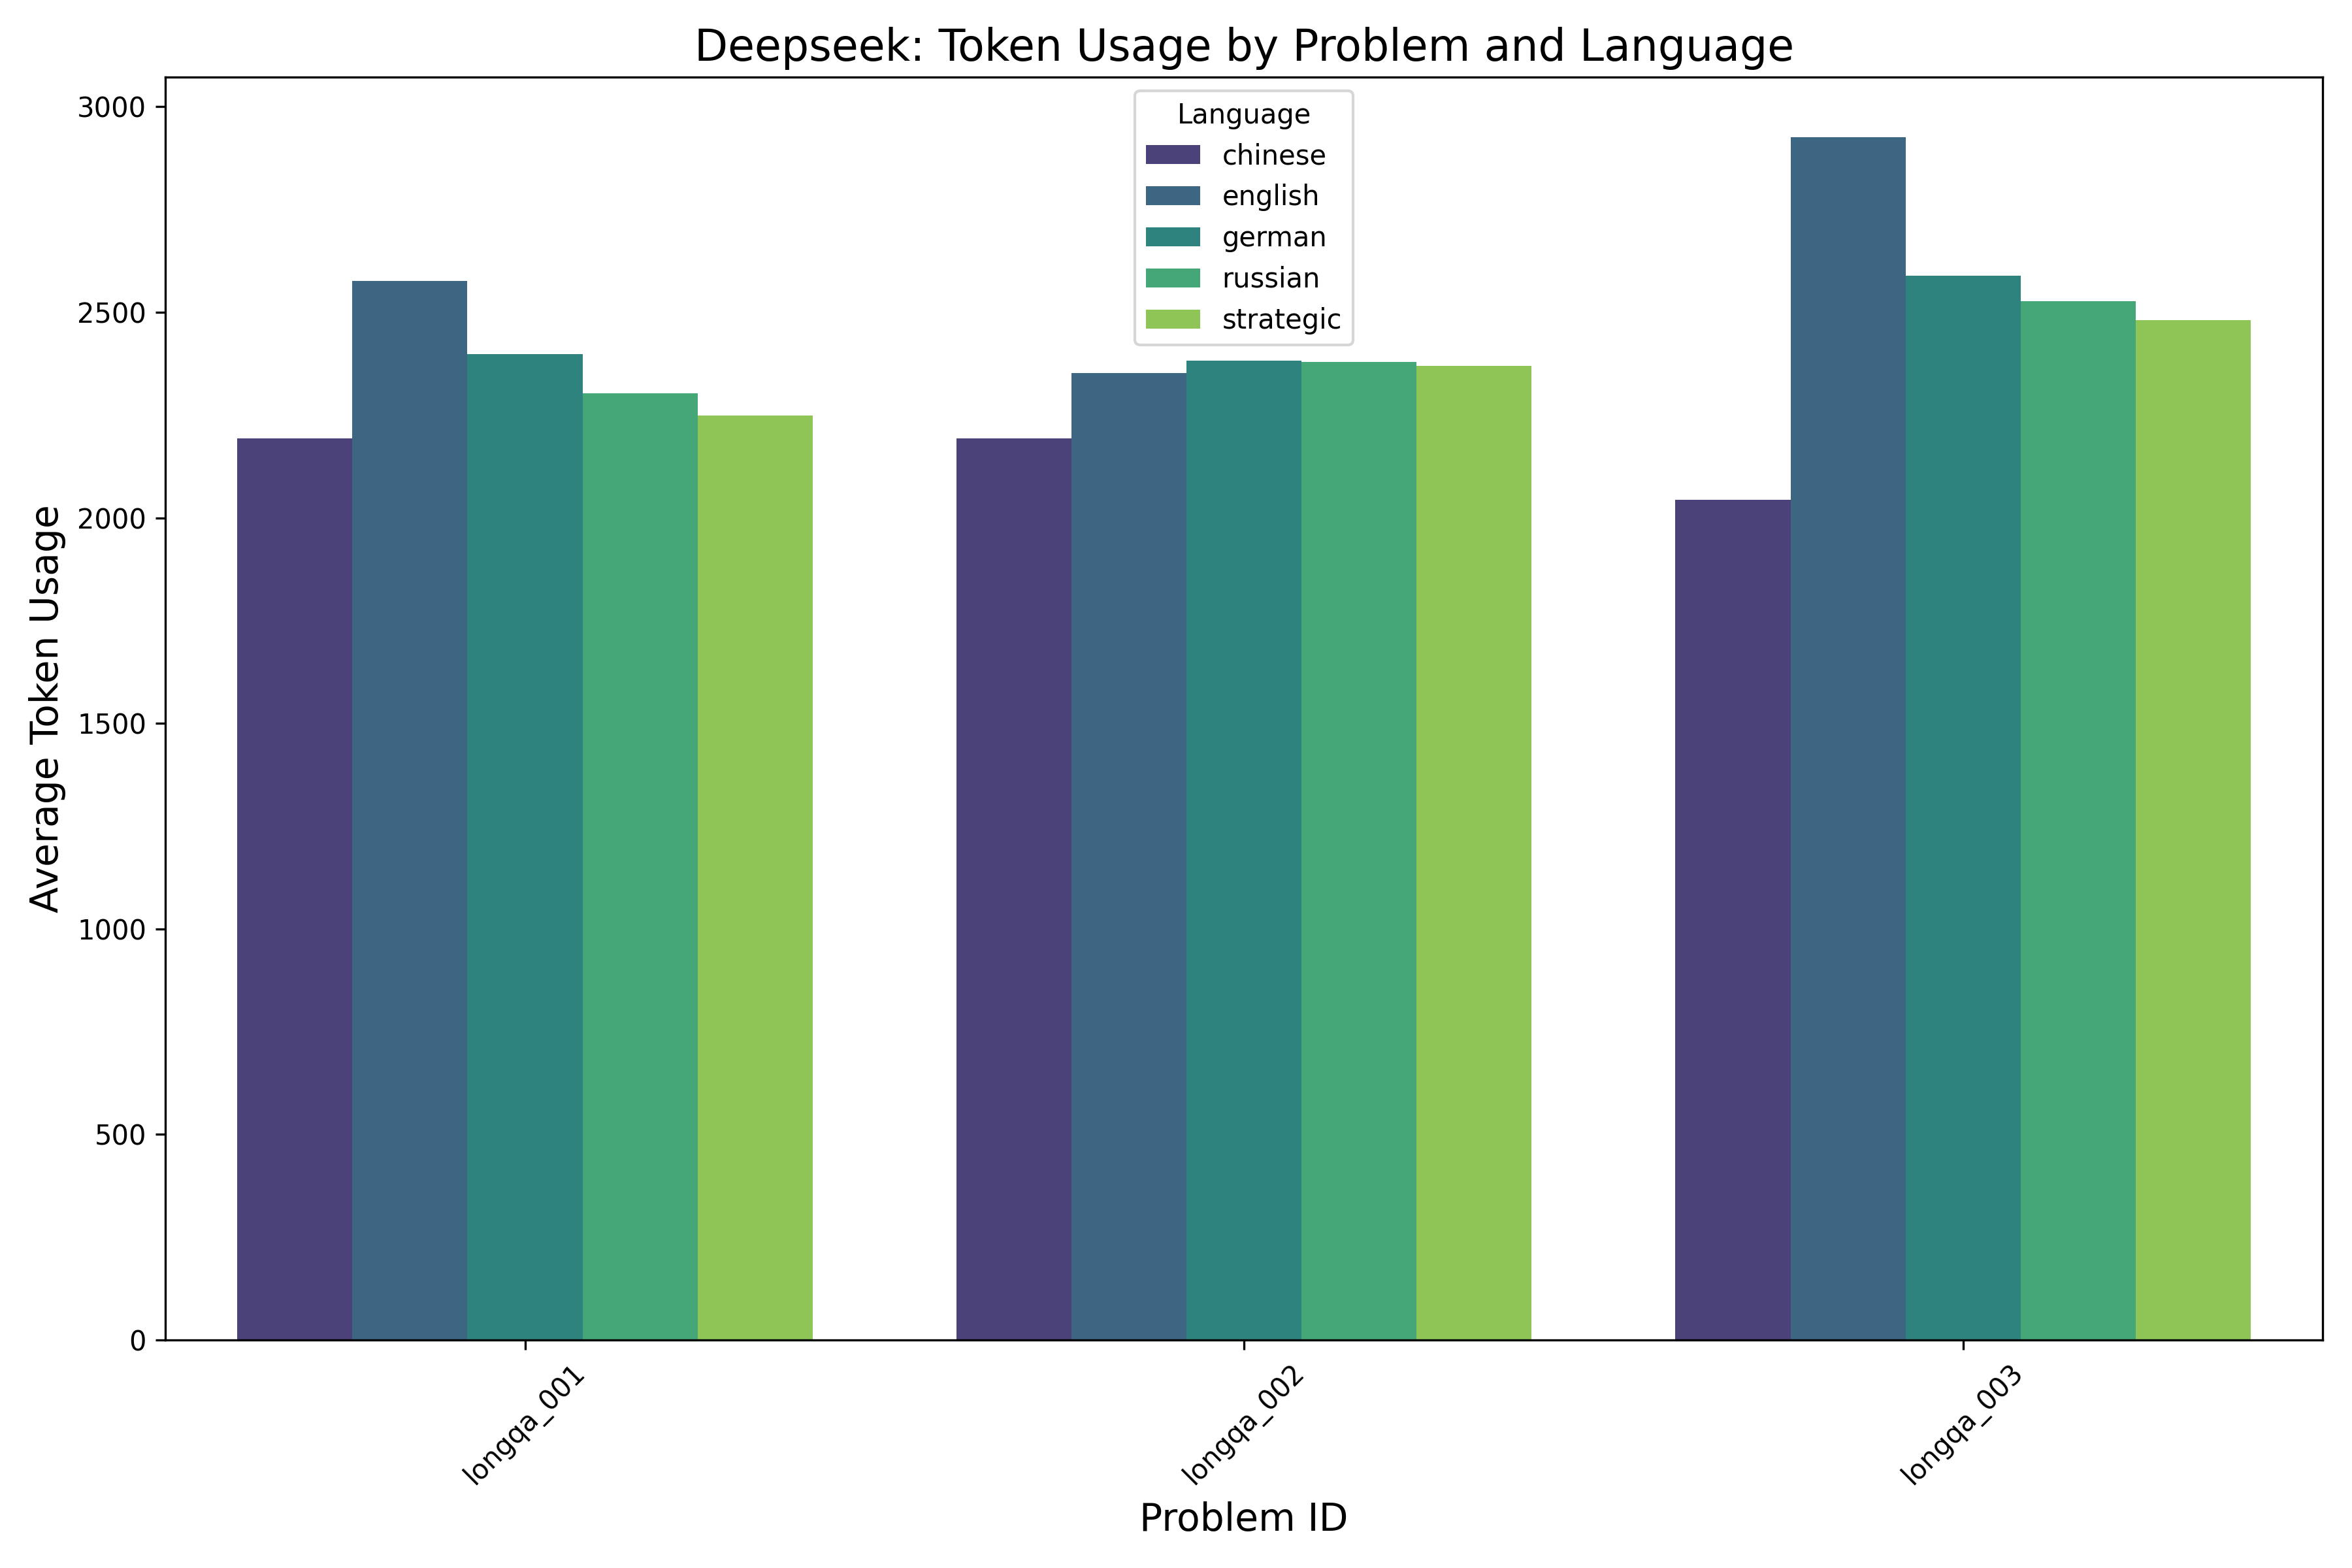
\includegraphics[width=0.9\textwidth]{visualizations/deepseek/deepseek_problem_tokens.png}
    \end{center}
    
    \begin{itemize}
        \item Chinese consistently uses fewer tokens across all problems
        \item Problem difficulty impacts relative efficiency of languages
        \item Strategic selection adapts to problem characteristics
        \item Token usage patterns consistent across different problems
    \end{itemize}
\end{frame}

\begin{frame}{Model Comparison: Anthropic vs. Deepseek}
    \begin{center}
        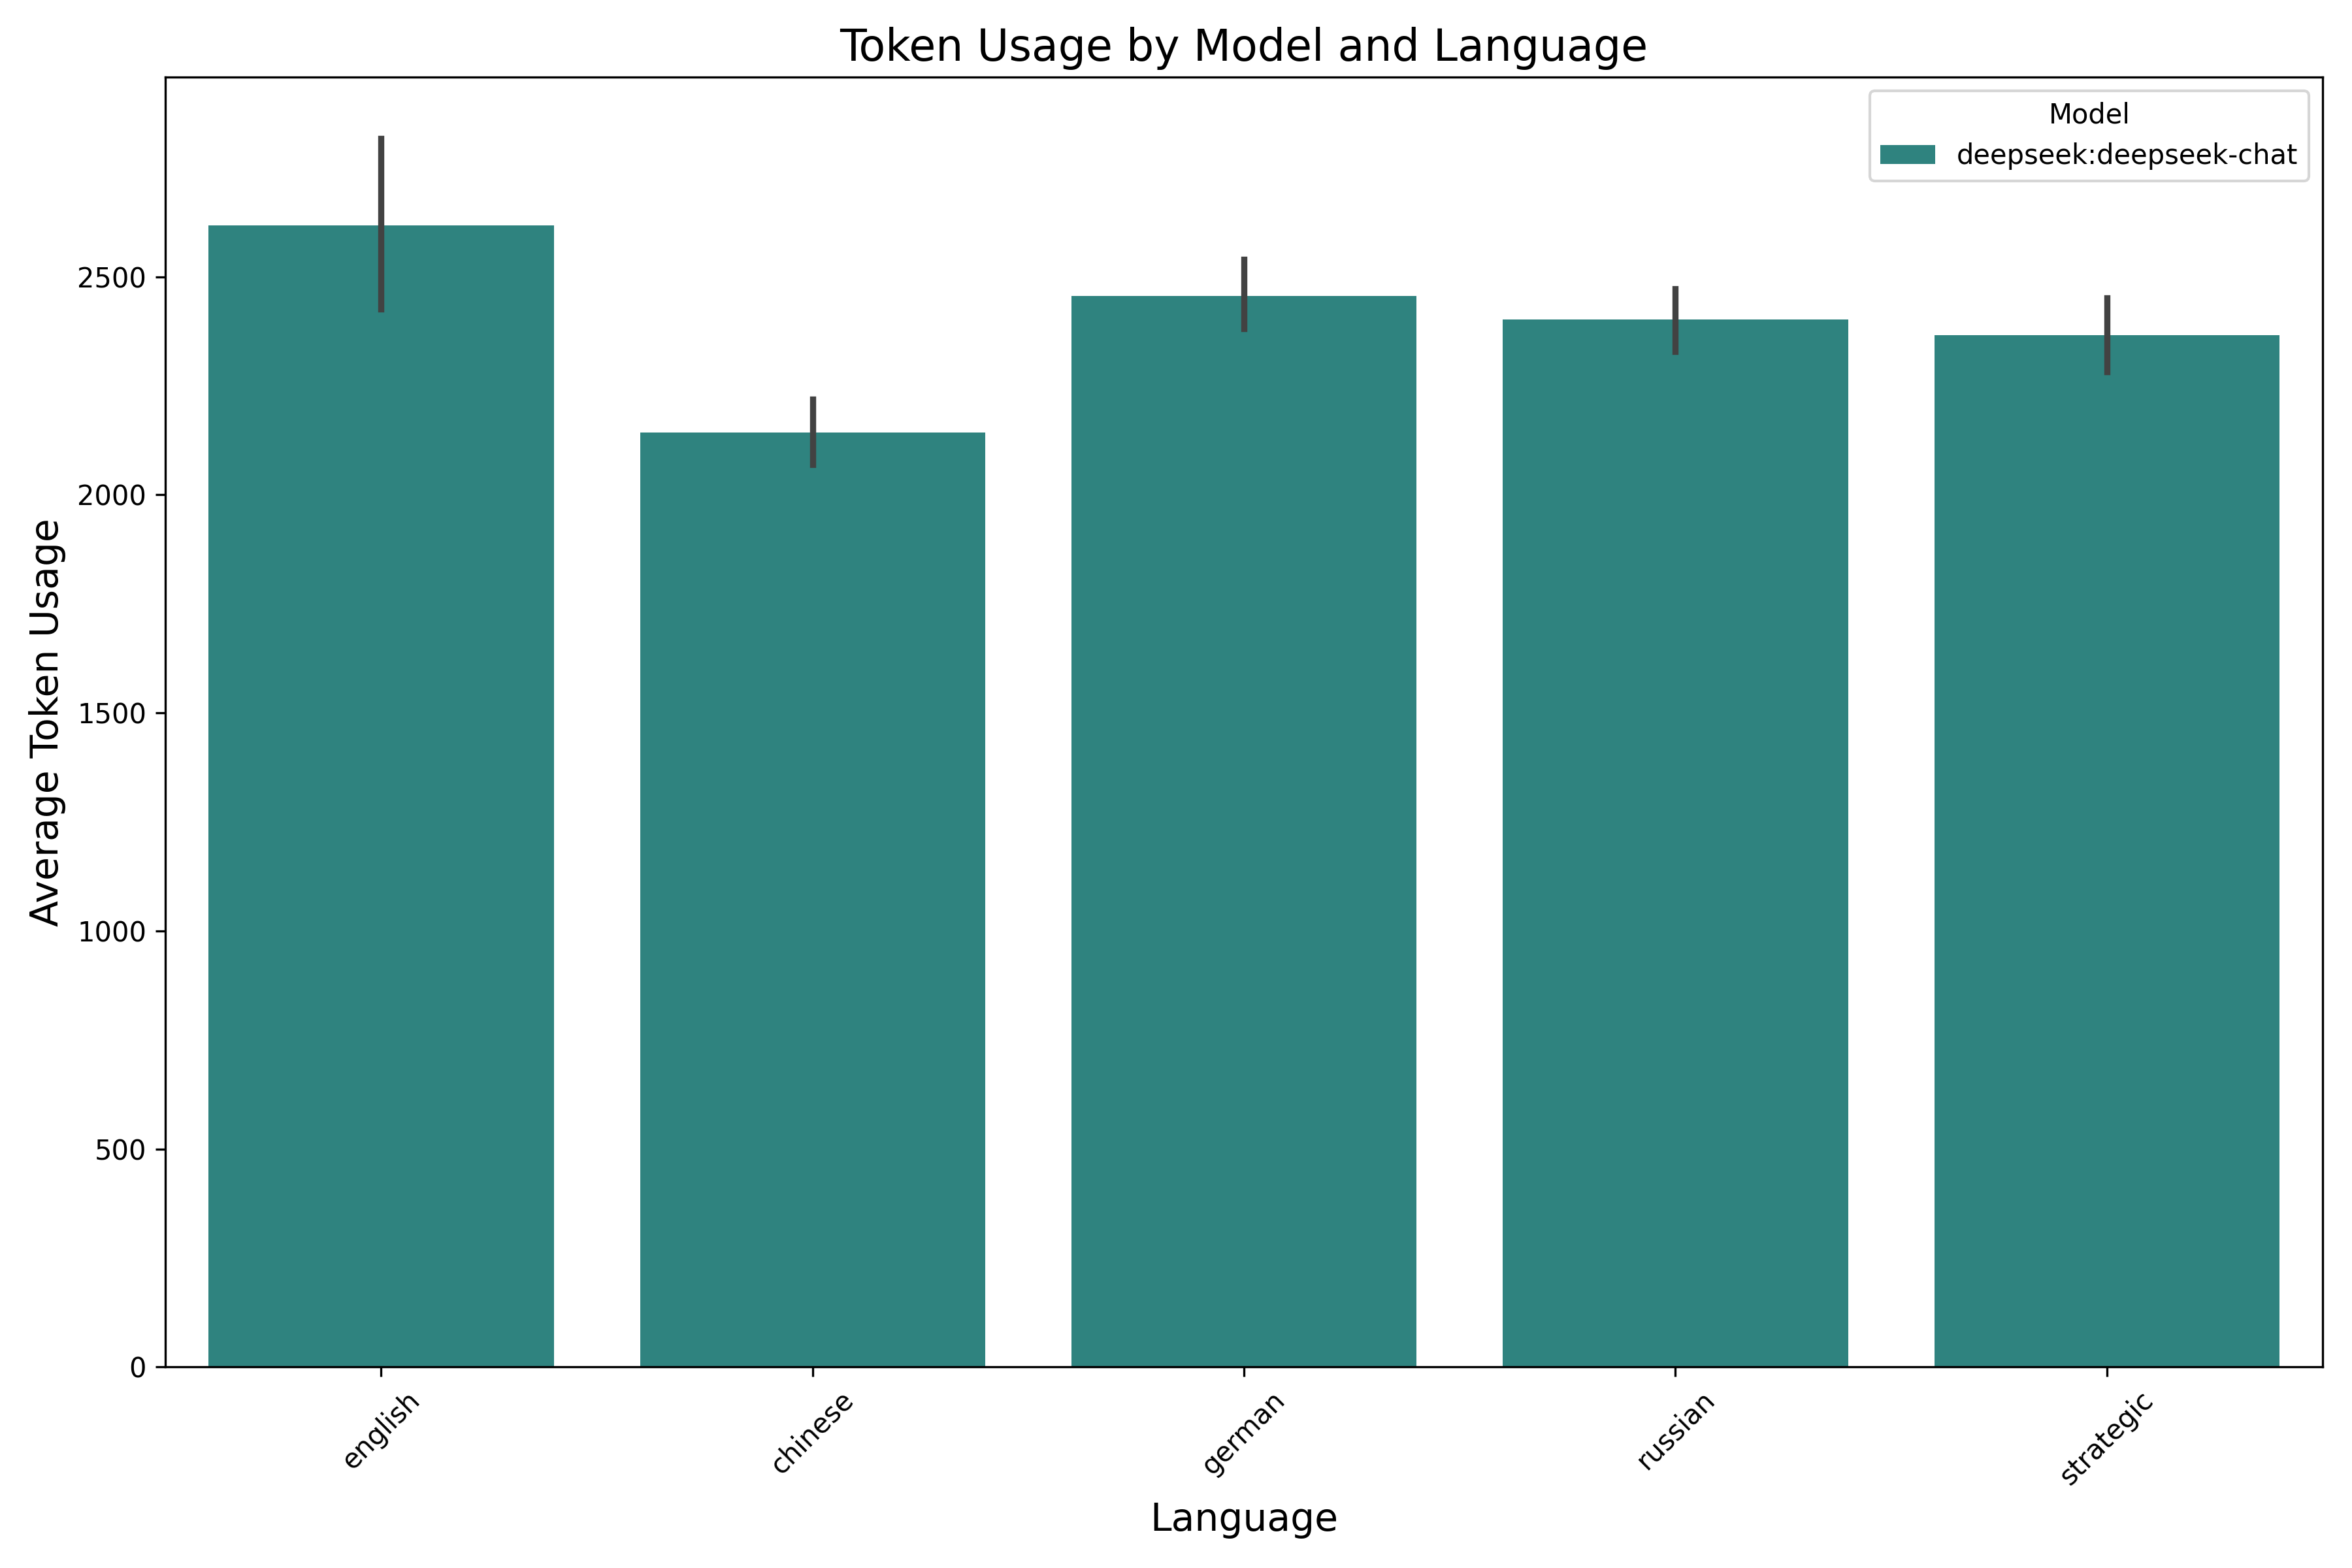
\includegraphics[width=0.9\textwidth]{visualizations/model_comparison/token_usage_by_model_language.png}
    \end{center}
    
    \begin{itemize}
        \item Deepseek shows similar language efficiency patterns to Anthropic
        \item Chinese consistently more efficient across both models
        \item Strategic language selection maintains efficiency advantage
        \item Deepseek shows higher efficiency gains for Chinese compared to Anthropic
    \end{itemize}
\end{frame}

\section{Practical Applications}

\begin{frame}{Domain-Specific Language Selection}
    \begin{columns}
        \column{0.5\textwidth}
        \textbf{Recommended Languages}
        \begin{itemize}
            \item Mathematical reasoning: Chinese (28.95\% savings)
            \item Logical reasoning: German (15.32\% savings)
            \item Scientific reasoning: Russian (12.76\% savings)
            \item Reading comprehension: English (baseline)
            \item Long-context QA: Strategic (1.92\% savings)
        \end{itemize}
        
        \column{0.5\textwidth}
        \textbf{Implementation Strategy}
        \begin{enumerate}
            \item Classify problem type and difficulty
            \item Select optimal language based on domain
            \item Perform reasoning in selected language
            \item Return answer in English
        \end{enumerate}
    \end{columns}
\end{frame}

\begin{frame}{Conclusions and Next Steps}
    \begin{block}{Key Conclusions}
        \begin{itemize}
            \item Language efficiency for chain-of-thought reasoning varies significantly by domain
            \item Chinese excels at mathematical reasoning but underperforms in long-context tasks
            \item Strategic language selection yields the highest overall efficiency
            \item Context length impacts language efficiency in complex ways
        \end{itemize}
    \end{block}
    
    \begin{block}{Next Steps}
        \begin{itemize}
            \item Complete Deepseek model testing across all benchmarks
            \item Develop more sophisticated language selection algorithms
            \item Explore hybrid approaches (domain-specific terms in English, reasoning in selected language)
            \item Test with additional models and languages
        \end{itemize}
    \end{block}
\end{frame}

\begin{frame}{Thank You}
    \begin{center}
        \Huge{Questions?}
        
        \vspace{1cm}
        \normalsize{Contact: research@kelaode.com}
    \end{center}
\end{frame}

\end{document}
